\documentclass[Main]{subfiles}
\begin{document}

\chapter{Mathematical Preliminaries}
%Intro
%-_-_-_-_-_-_-_-_-_-_-_-_-_-_-_-_-_-_-_-_-_-_-_-_-_-_-_-_-_-_-_-_-_-_-_-_-_-_-_-_-_-_-_-_-_-_-_-_-_-_-_-_-_-_-_

	\begin{Warning}
		Le interazioni matematiche sono complesse  e non triviali (vedi un po' di articoli di introduzione a AQFT per ispirarti)
		
		Tendenzialmente le teorie quantistiche di campi moderne sono di Quantizzazione.. Quindi richiedono di specificare bene la struttura del campo classico (vedi intro di Mangiaratti shardashivly)
		
		Gli strumenti matematici per raccontare la teoria dei campi classici sono essenzialmente 3: Fibrati, S-T G-H, LDOP e GHOP.
		
		IN questo paper non ci soffermeremo sulle strutture del framework puramente quantistico (* algebre e quant'altro). Per un primer vedere articolo di Dappiaggi o Libro Adv aqft.
		
		Diamo per scontato un background di base in Geometria differenziale e derivate esterne (algebre di Grassman? global calculus? non so come chiamarlo!).
		
		Potrei avere la tentazione a provare ad usare un po' di linguaggio basilare delle categorie... la mia fonte è \href{http://katmat.math.uni-bremen.de/acc/acc.pdf}{Joy of Cat}.
	\end{Warning}
	
	\begin{Warning}
		Stile: Intro lapiadaria ai 3 argomenti ( bundle cinematica di campo, Glob iper stage per descrivere dinamica di tipo propagativo, Operatori tipo onda). Poi smitragliata di definizioni come faceva Penati.
	\end{Warning}	


%-_-_-_-_-_-_-_-_-_-_-_-_-_-_-_-_-_-_-_-_-_-_-_-_-_-_-_-_-_-_-_-_-_-_-_-_-_-_-_-_-_-_-_-_-_-_-_-_-_-_-_-_-_-_-_
%-_-_-_-_-_-_-_-_-_-_-_-_-_-_-_-_-_-_-_-_-_-_-_-_-_-_-_-_-_-_-_-_-_-_-_-_-_-_-_-_-_-_-_-_-_-_-_-_-_-_-_-_-_-_-_
	\section{Fiber Bundles}
		\danger intro
		
		\subsection{Formal Definition}
			Although it would be possible to present the concept \emph{bundle} in a more general way through the language of categories, for our argument will be sufficient to consider only the case of \emph{smooth bundles}.

			\begin{definition}[Fiber Bundle]\label{Def:SmoothBundle}
				A \emph{Fiber Bundle} consists in a 4-ple $(E,M,Q,\pi)$ where:
				\begin{itemize}
					\item[-] $E,M,Q$ :  smooth manifolds called respectively \emph{Total Space}, \emph{Base Space}, \emph{Typical Fiber}.
					\item[-] $\pi : E \rightarrow M $ continuous smooth function (called \emph{Bundle Projection})
				\end{itemize}
				Endowed with a \emph{Local Trivialization}:
				\begin{itemize}
					\item $\forall x \in E$ $\exists$ a couple $(U, \chi)$ (called \emph{local trivialization})
					\begin{itemize}
						\item $U$ : neighborhood of $x$
						\item $\chi$ :$\pi^{-1}(U) \rightarrow U \times Q$ : diffeomorphism
							%DaRivedere
 							\footnote{surjectivity $\Rightarrow$ $\pi^{-1}(U) \neq \emptyset$.} 
 							\footnote{cartesian product of topological space is a topological space with the direct product topology.}
					\end{itemize}
					such that: $p_1 \cdot \chi = \pi \vert_{\pi^{-1}(p)}$.

					i.e: the following graph commutes:
					\begin{tikzpicture}
						 \matrix (m) [matrix of math nodes,row sep=3em,column sep=4em,minimum width=2em] {
     						\pi^{-1}(U) & U \times Q \\
     						U &  \\};
 						 \path[-stealth]
 							(m-1-1) edge node [left] {$\pi$} (m-2-1)
            				edge [right] node [above] {$\chi$} (m-1-2)
    						(m-1-2) edge [right] node [below] {$p_{1}$} (m-2-1);;
					\end{tikzpicture}

				\end{itemize}
			\end{definition}

			\begin{figure}[h!]
  				\caption{The complete fiber bundle Structure.}
  				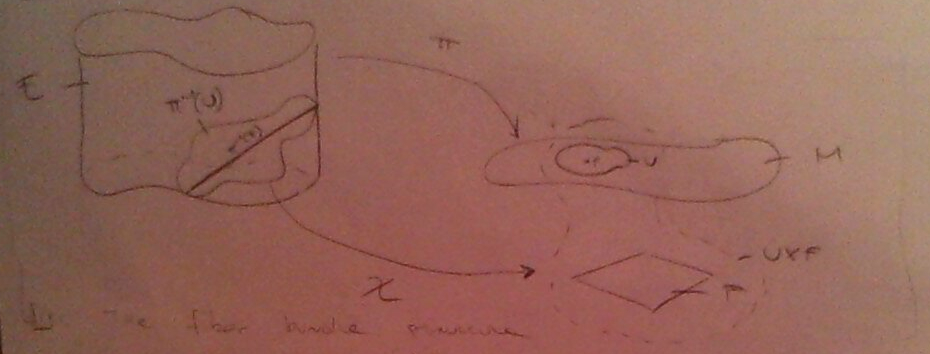
\includegraphics[width=0.5\textwidth]{Pictures/FiberBundle}
  				\centering
			\end{figure}
			\begin{notationfix}
				It is customary to refer to a vector bundle specifying only its total space:
				\begin{displaymath}
					\gls{Bundle}%E= ( E,\pi, B ; F)
				\end{displaymath}
			 	In the following we adopt this convention whenever this does not lead to misunderstandings.
			\end{notationfix}
			
			\begin{observation}
				For all $p\in M$ we refer to the submanifold $E_{p} := \pi_{-1}(p) \subset E $ as \emph{fiber over the point p}.
				\\
				Every fiber $E_p$ is diffeomorphic to the typical fiber $F$ through the local trivialization charts.
			\end{observation}
			
			\begin{notationfix}
				We say that a smooth bundle E is \emph{(globally) trivial} if $E \simeq M \times Q$ i.e there exists a trivialization of $E$ which is defined everywhere.
				Note that definition \ref{Def:SmoothBundle}  prescribes the existence of local trivializations only.
			\end{notationfix}
			
			When a smooth fiber bundle $(E,\pi,M;Q)$ is considered, in addition to the typical functions of the bundle $(\pi, \chi_{\alpha})$ should be taken in account also  the local charts $(U_{\alpha_k}, \phi_{\alpha_k})_{k = E,M,Q}$ provided by the atlases of $E,M$ and $Q$:
			\begin{definition}[Bundle atlas]
				Collection local chart which trivializes $E$. I.e. triples  $(U_\alpha, \psi_\alpha, \chi_\alpha)$ where:
				\begin{itemize}
					\item $U_\alpha$ open set in $M$ such that $\bigcup_{\alpha} U_{\alpha} \supseteq M$.
					\item $\chi_\alpha$  is a local trivialization.
					\item $(U_\alpha,\psi_\alpha)$ local chart on $E$ constructed from charts on the base and fiber manifold:
						\begin{displaymath}
							\psi^{(E)}_\alpha = \psi_\alpha^{(M)} \times  \psi_\alpha^{(Q)} \circ \chi_\alpha
						\end{displaymath}	
				\end{itemize}		
			\end{definition}
			
			
						
			Endowing the bundles manifolds with other additional structures, can be introduced important subclasses of smooth bundles:
			\begin{definition}[Vector Bundle]
				Is a smooth bundle $E=(E,\pi,M;V)$ such that:
				\begin{itemize}
					\item The typical fiber manifold $V$ is a finite dimensional vector space.	
					\item All the trivialization $\chi_{\alpha} $ are diffeomorphism such that:
						\begin{displaymath}
							\chi_{\alpha}\vert_{\pi^{-1}(p)} \in \mathbb{GL}(n, \mathbb{R})
						\end{displaymath}
				\end{itemize}
			\end{definition}

		\subsection{Cross Sections}
			The notion of bundle is particularly interesting from the perspective of physics because provides the rigorous description of a $Q-$valued field over the space $M$:			
			\begin{definition}[Smooth Section]
				Function $\phi : M \rightarrow E$ such that:
					\begin{itemize}
						\item $\phi$ smooth.
						\item $\phi \cdot \pi = \Id_M$ 
					\end{itemize}
			\end{definition}
			
			\begin{notationfix}
				We refer to:
					\begin{itemize}
						\item \emph{Global section} $\Leftrightarrow$ $\textrm{dom}(\phi) = B$
						\item \emph{Local section} $\Leftrightarrow$ $\textrm{dom}(\phi) \subset B$ \footnote{Usually the domain is an open set of B)}
					\end{itemize}
				We denote the set of all the smooth sections of the bundle $E$  as:
				\begin{displaymath}
					\gls{Sections}
				\end{displaymath}
			\end{notationfix}
			
			\begin{observation}
				In general, \gls{Sections} is an infinite dimensional manifolds. In case of vector bundle is also a linear space, and the section are called "vector fields".
			\end{observation}
			
			
		\subsection{Mapping between Bundles}
			%Bundle morphism
			Consider two smooth bundles $E=(E,\pi,M; Q)$ and $E'=(E',\pi',M; Q')$ on the same base space $M$.
			\begin{definition}[Bundle map (\emph{Fiber Preserving map})]\label{Def:BundleMap}
				Smooth function $\phi: E \rightarrow E'$ such that:			
			 	\begin{displaymath}
			 		\phi(E_{x})= F_{x} \qquad \forall x \in M.
			 	\end{displaymath}
				i.e.:
				\begin{tikzpicture}
					 \matrix (m) [matrix of math nodes,row sep=3em,column sep=4em,minimum width=2em] {
						E & & F \\
       					& M & \\};
					\path[-stealth]
    					(m-1-1) edge node [left] {$\pi_{E}$} (m-2-2)
   		         		edge [right] node [above] {$\phi$} (m-1-3)
    					(m-1-3) edge node [right] {$\pi_{F}$} (m-2-2);
				\end{tikzpicture}
			\end{definition}
			\begin{observation}
				Definition \ref{Def:BundleMap} is a special case of \emph{Bundle-morphism}. (see for example \cite{G.Sardanashvily2013})
			\end{observation}

			%pullback bundle
			Consider a smooth manifold $N$, a (smooth) fiber bundle $E=(E,\pi,M;Q)$, and a smooth function $f: N \rightarrow M$. It's possible to induce\cite{Husemoller} a bundle structure from the manifold $M$ to $N$:
			\begin{definition}[Pull-Back Bundle]
				3-ple $f^* (E) = (f^* (E) =, \pi^*,N)$ such that:
				\begin{itemize}
					\item $f^* (E) =  \big\{ (b',e) \in N \times E \quad \big\vert \; f(b') = \pi(e) \big\} $
					\item $\pi^*:f^* (E) \rightarrow N $ such that $ \pi* (b',e) = \textrm{pr}_1 (b',e)= b' $
				\end{itemize}
				\begin{tikzpicture}
					\matrix (m) [matrix of math nodes,row sep=3em,column sep=4em,minimum width=2em] {
						f^* E & E \\
						N & M \\};
						\path[-stealth]
    						(m-1-1)edge node [left] {$\pi'$} (m-2-1)
    						(m-1-2) edge node [right] {$\pi$} (m-2-2)
    						(m-2-1) edge [right] node [above] {$f$} (m-2-2);
				\end{tikzpicture}
			\end{definition}
			\begin{proposition}
				$f^* (E) = (f^* (E) =, \pi^*,N)$ consitute a fiber bundle of typical fiber Q.
			\end{proposition}
			\begin{proof}
				To complete the fiber bundle structure is sufficient to provide a local trivialization atlas.
				\\
				$\forall ( U, \phi)$ local trivialization on $(E, \pi, M)$  consider $\psi: f^* E \rightarrow N \times Q$ such that $\psi( b',e) = \bigg( b', pr_2 \big( \phi(e)\big)\bigg)$.
				\\
				Then $(f^{-1}(U),\psi)$ is a local trivialization of the pull-back bundle and the fiber of $f^*E$ over a point $b′\in B'$  is just the fiber of E over $f(b′)$.
			\end{proof}

			
			%mor bundle
			It is also noteworthy that, given any two vector bundles $E =(E\pi,M,Q)$ and $E =(E'\pi,M',Q')$, we can construct 	naturally a third fiber bundle.
			Consider $\hom(E,E')$ the set of all the fiber preserving map between the two bundles:
			\begin{definition}[Bundle of morphisms]
				Fiber bundle $\hom(E,E')$ over the base space $M$ such that the fiber over a base point $p\in M$ is the infinite dimensional manifold $\hom(E_p,E'_p)$ isomorphic to $\hom(Q,Q')$.
			\end{definition}
			\begin{notationfix}
				We shall write $End(E)$ for $\hom(E,E)$ and call it bundle of endomorphism, whose typical fiber is $\textrm{End}(Q)$.
			\end{notationfix}
			\begin{remark}
				If $F,F'$ are vector bundle then the fiber of  $\hom(F,F')$ over a base point $p\in M$ is $\hom(F_p,F'_p)$, which is a vector space isomorphic to the vector space $\hom(V,V')$ of linear applications from $V$ to $V'$
			\end{remark}
	
		\subsection{Tangent Bundles}
			The \emph{tangent} bundle is a natural structure defined on any smooth manifold, represent the canonical example of  non-trivial vector bundle.
						
			\begin{definition}[Tangent Bundle]
				The smooth vector bundle $TM=(TM,\tau,M;\Real^m)$ such that:
				\begin{itemize}
					\item The total space is the union of all tangent spaces to 
						$$M: TM \coloneqq \underset{p \in M}{\sqcup} T_pM  \equiv \bigcup_{x\in M} {x}\times T_x M$$
					\item The bundle projection maps each tangent vector $v\in  T_pM$ to the correspondent base point  $p$;
						$$\tau : (p,v_p) \mapsto p $$
				\end{itemize}
			\end{definition}			
			
			\begin{observation}
				In a similar fashion it's possible to construct a vector bundle relatively to any tensor product of the tangent spaces.
				i.e.:
				\begin{itemize}
					\item \emph{Cotangent Bundle} $T^*M$ is build by disjoint union of the dual tangent space: 
					$$T_p^*M \; \forall p\in M$$
					\item \emph{Tensor Bundle} $T^{(k,l)}M$ is build by disjoint union of the tensor product of tangent space with itself:
					\begin{displaymath}
						T^{(k,l)}_ p M = \underbrace{T^*_pM \otimes \cdots \otimes T^*_pM}_{\textrm{k-times}} \otimes
						\underbrace{T_pM \otimes \cdots \otimes T_pM}_{\textrm{l-times}}
					\end{displaymath}
					\item \emph{k-forms Bundle} $ \bigwedge^m( T^*M)$ is build by disjoint union of the antisimmetrized tensor product of the dual tangent space with itself.
				\end{itemize}
			\end{observation}
			
			
			\subsubsection{Tautological one-form and simplectic form.}
					\begin{notationfix}
						In the context of Classical mechanics is customary to refer to the cotangent bundle $T^*Q$ over the smooth manifold  $Q $ - called \emph{Configuration Space}  - as \emph{Phase Space}.
					\end{notationfix}
					Since $TQ$ and $T^*Q$ are diffeomorphic , it might seem that there is no particular reason in treating this two spaces separately, but it is not so.
					There are certain geometrical objects that live naturally on $T^*Q$ , not on $TQ$.\\
					Of greatest interest in mathematical-physics are the Poincarè forms\cite{Fraenkel}.
	
					Consider a smooth manifold $Q$ and call $\Phase=T^*Q$ the corresponding cotangent bundle.
					\begin{definition}[Tautological (Poincare) 1-form]
						Is the 1-form over $\Phase$:
						\begin{displaymath}
							\theta_0 \in \Gamma^\infty (T^*\Phase)
						\end{displaymath}
					such that the action on a generic point $ \omega_{\alpha_p} \in T_{\alpha_p}M$ ( in the fiber of $\alpha_p$, which in turn is a one-form on the fiber of $p\in Q$) is given by:
						\begin{displaymath}
						\theta_0 \big(\alpha_p \big): T_{\alpha_p}\Phase \rightarrow \Real \qquad : \; \omega_{\alpha_p} \mapsto \alpha_q \circ T \tau^*_Q \big( \omega_{\alpha_p} \big)
						\end{displaymath}
					\end{definition}
					\begin{figure}[h!]
   						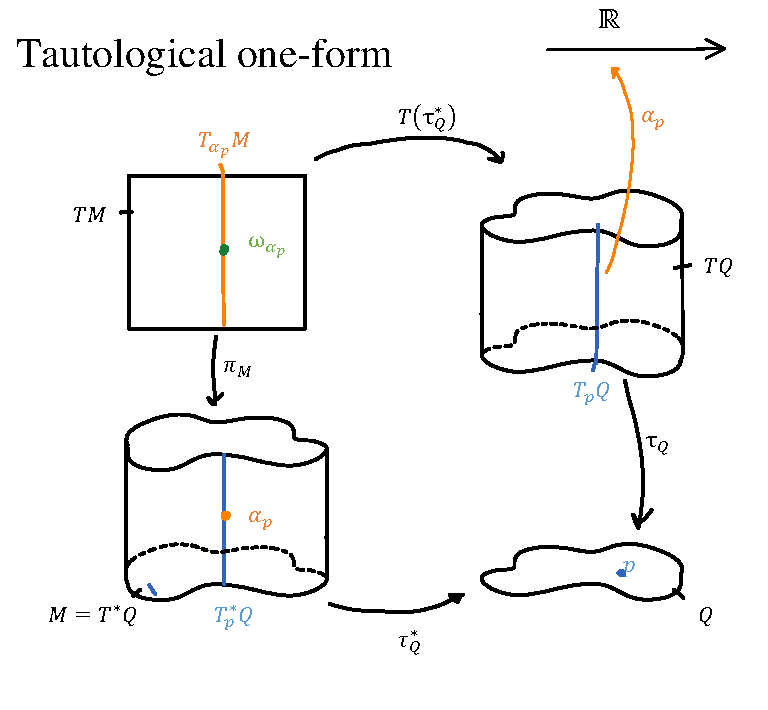
\includegraphics[width=0.5\textwidth]{Pictures/Tautological1Form} 
 						\caption{The definition of tautological 1-form is achieved exploiting the concept of \emph{Tangent map} and remembering that $\alpha_p: T_p \Phase \rightarrow \Phase$ is a linear functional.} 
  						\centering
					\end{figure}	
	
					\begin{notationfix}
						Canonical coordinates are defined as a special set of coordinates on the cotangent bundle of a manifold. 
						They are usually written as a set of $(q^i,p_j)$ where ${q_i}$ are denoting the coordinates on the underlying manifold and the ${p_j}$ are denoting the conjugate momentum, which are decomposition of 1-forms in $T_p^*M$ on the dual natural basis $d q^J$ in the cotangent bundle at point $q$ in the manifold.
					\end{notationfix}
	
					\begin{observation}
						In canonical coordinate the tautological one-form assumes the famous expression:
						\begin{displaymath}
							\theta_0 = \sum_{i=1}^n {p_i} d q^i
						\end{displaymath}
						(note that $d q^i$ is a 1-form on $T^*M$ calculated with respect to the coordinate on the bundle. Has not to be confused with the 1-natural form $d q^i \in T^*_p M$.)
					\end{observation}
	
					The claim is proved by the following definition:
					\begin{definition}[Canonical (Poincare)  symplectic form]
						Symplectic form:
						\begin{displaymath}
							\omega_0 \coloneqq -d \theta_0
						\end{displaymath}
						In canonical coordinates assumes the famous expression:
						\begin{displaymath}
							\omega_0 \coloneqq \sum_{i=1}^n  d q^i \wedge d p_i
						\end{displaymath}
					\end{definition}
					
		\subsection{Jet Bundles}
			The jet bundle is a certain construction that makes a new smooth fiber bundle out of a given smooth fiber bundle. 			
			The first step is to identify the typical fiber for this construction.
			\\
			Suppose $M$ is an m-dimensional manifold and that $(E, \pi, M)$ is a fiber bundle.Consider the set of all the local sections whose domain contains $p$:
			\begin{displaymath}
				\Gamma^\infty (p) \coloneqq \big\{ \sigma \in \Gamma^\infty(E) \quad \big\vert\:  p \in \dom(\sigma)  \big\}
			\end{displaymath}

			We define an equivalence relation between such section \emph{up to r-th order}:
			\begin{definition}[r-jet equivalence]
				Two such section $\sigma, \eta \in \Gamma^\infty(p)$ have the \underline{same \emph{r-jet} at $p$} $(\sigma \sim \eta)$ 
				iff:
				\begin{displaymath}
					\left.\frac{\partial^{|I|} \sigma^{\alpha}}{\partial x^{I}}\right|_{p} = \left.\frac{\partial^{|I|} \eta^{\alpha}}{\partial x^{I}}\right|_{p} 
					\quad \forall I\in \Natural^m_0 \, \vert \, 0 \leq |I| \leq r.
				\end{displaymath}	
				where $I$ is a \emph{Multi-index}.	
			\end{definition}
			\begin{remark}
				(Multi-index notation)
				\\
				A multi-index is a natural valued finite dimensional vector  $I=(i_1, i_2, \ldots, i_m)\: \in \Natural^m_0$ with $m<\infty$.
				\\
				On $\Real^n$ a general differential operator can be identified by a multi-index:
				\begin{displaymath}
					\frac{\partial^{|I|}}{\partial x^{I}} := \prod_{i=1}^{m} \left( \frac{\partial}{\partial x^{i}} \right)^{I(i)}
				\end{displaymath}
				(Until the Schwartz theorem holds, the order of derivation is irrelevant.)
				\\
				The order of the multi-index is defined as:
				\begin{displaymath}
					|I| := \sum_{i=1}^{m} I(i)
				\end{displaymath}
			\end{remark}
	
			We define the \emph{r-th Jet in p} as the equivalence class under this relation.
			\begin{definition}[Space of r-th Jet in p]
				\begin{displaymath}
					J^r_{\,p}(E) \coloneqq \frac{\Gamma^\infty(p)}{\sim}
				\end{displaymath}
				where $\sim$ is the r-Jet equivalence.
			\end{definition}
			\begin{notationfix} 
				A r-jet with representative $\sigma$ is denoted as $j^r_p\sigma$ . 
				\\
				The integer $r$ is also called the order of the jet, $p$ is its source and $\sigma(p)$ is its target.
			\end{notationfix}
	
			Glueing all the jet fiber $J^r_p (E)$ together for all the base point $p\in M$, as done for the tangent bundle,  
			we obtain the desired bundle:
			\begin{definition}[r-th Jet Bundle of $E$]
				The smooth bundle $(J^r(E), \pi_r, M)$	where:
				\begin{itemize}
					\item $J^r(E) \coloneqq \underset{p \in M}{\sqcup} J^r_p (E)
						 \equiv \big\{j^r_p\sigma \quad \vert \; p\in M, \; \sigma \in \Gamma^\infty(p) \big\}$
					\item $\pi_r: J^r(E) \rightarrow M$ such that $j^{r}_{p}\sigma \mapsto p $
				\end{itemize}
			\end{definition}

%-_-_-_-_-_-_-_-_-_-_-_-_-_-_-_-_-_-_-_-_-_-_-_-_-_-_-_-_-_-_-_-_-_-_-_-_-_-_-_-_-_-_-_-_-_-_-_-_-_-_-_-_-_-_-_
%-_-_-_-_-_-_-_-_-_-_-_-_-_-_-_-_-_-_-_-_-_-_-_-_-_-_-_-_-_-_-_-_-_-_-_-_-_-_-_-_-_-_-_-_-_-_-_-_-_-_-_-_-_-_-_
	\section{Globally Hyperbolic Spacetimes}
			\begin{Warning}
				Mettere solo le definizioni che uso prese dagli articoli di review delle Fonti
			\end{Warning}	
			Appunti che mi ero preso scrivendo il secono capitolo:
					
			This condition is strictly connected to the dynamic behaviour of the system.
		\subsection{A reprise in Spacetimes Geometry}	
		Recurring definitions in general Relativity (excluding the general smooth manifold prolegomena).

	\begin{definition}[Space-Time]
		A quadruple $(M, g, \mathfrak{o}, \mathfrak{t})$ such that:
		\begin{itemize}
			\item $(M,g)$ is a time-orientable n-dimensional manifold $(n>2)$
			\item $\mathfrak{o}$ is a choice of orientation
			\item $\mathfrak{t}$ is a choice of time-orientation
		\end{itemize}
	\end{definition}

	\begin{definition}[Lorentzian Manifold]
		A pair $(M, g)$ such that:
		\begin{itemize}
			\item $M$ is a n-dimensional $(n\geq2)$, Hausdorff, second countable, connected, orientable smooth manifold.
			\item $g$ is a Lorentzian metric.
		\end{itemize}
	\end{definition}
			
	\begin{definition}[Metric]
		A function on the bundle product of $TM$ with itself: $$g: TM \times_M TM \rightarrow \Real$$ such that the restriction on each fiber $$g_p: T_pM \times T_pM \rightarrow \Real $$ is a non-degenerate bilinear form.
	\end{definition}
	
	\begin{notationfix}
		 \begin{itemize}
		 	\item \emph{Riemman} if the sign of $g$ is positive definite, \emph{Pseudo-Riemman} otherwise.
		 	\item \emph{Lorentzian} if the signature is $(+, -, \ldots,- )$ or equivalently $(-,+,\ldots,+)$.
		 \end{itemize}
	\end{notationfix}

	\begin{observation}[Causal Structure]
		If a smooth manifold is endowed with a Lorentzian manifold of signature $(+, -, \ldots, -)$ then the tangent vectors at each point in the manifold can be classed into three different types. 
		\begin{notationfix}
			$\forall p \in M, \quad \forall X \in T_pM$, the vector is:
			\begin{itemize}
				\item \emph{time-like} if $g(X,X)>0$.
				\item \emph{light-like} if $g(X,X)=0$.
				\item \emph{space-like} if $g(X,X)<0$.
			\end{itemize}
		\end{notationfix}
	\end{observation}

	\begin{observation}[Local Time Orientability]
		$\forall p\in M$ the timelike tangent vectors in $p$ can be divided into two equivalence classes taking
		\begin{displaymath}
			X \sim Y \; \textrm{iff} \; g(X,Y)>0 \qquad \forall X,Y \in T^\textrm{time-like}_pM:
		\end{displaymath}
		We can (arbitrarily) call one of these equivalence classes "future-directed" and call the other "past-directed". Physically this designation of the two classes of future- and past-directed timelike vectors corresponds to a choice of an arrow of time at the point. The future- and past-directed designations can be extended to null vectors at a point by continuity.
	\end{observation}
	
	\begin{definition}[Time-orientation]
		A global tangent vector field  $\mathfrak{t}\in \Gamma^\infty(TM)$ over the Lorenzian manifold $M$ such that:
		\begin{itemize}
			\item $\supp(\mathfrak{t}) = M$
			\item $\mathfrak{t}(p)$ is time-like $\forall p \in M$.
		\end{itemize}
	\end{definition}
	\begin{observation}
		The fixing of a time-orientation is equivalent to a consistent smooth choice of a local time-direction.
	\end{observation}	
	
	\begin{definition}[Time-Orientable Lorentzian Manifold]
		A Lorentzian Manifold $(M,g)$ such that exist at least one time-orientation $\mathfrak{t}\in \Gamma^\infty(TM)$.
	\end{definition}

	\begin{notationfix}
		Consider a piece-wise smooth curve $\gamma: \Real\supset I \rightarrow M$ is called:
		\begin{itemize}
			\item \emph{time-like} (resp. light-like, space-like) iff $\dot{\gamma}(p)$ is time-like (resp. light-like, space-like) $\forall p \in M$.
			\item \emph{causal} iff $\dot{\gamma}(p)$ is nowhere spacelike.
			\item \emph{future directed} (resp. past directed) iff is causal and  $\dot{\gamma}(p)$ is future (resp. past) directed $\forall p \in M$.
		\end{itemize}
	\end{notationfix}

	\begin{definition}[Chronological $\substack{\textrm{ future}\\ \textrm{past } }$ of a point]
		Are two subset related to the generic point $p	\in M$:
		\begin{displaymath}
			\mathbf{I}_M^\pm(p) \coloneqq \big\{ q \in M \big\vert \; \exists \gamma \in C^\infty\big((0,1), M\big)\;  \textrm{\footnotesize time-like } \substack{\textrm{future}\\ \textrm{past} } -\textrm{\footnotesize directed }:\; \gamma(0)=p,\; \gamma(1)=q  \big\}
		\end{displaymath}
	\end{definition}
	
	\begin{definition}[Causal $\substack{\textrm{ future}\\ \textrm{past } } $ of a point]
		Are two subset related to the generic point $p	\in M$:
		\begin{displaymath}
			\mathbf{J}_M^\pm(p) \coloneqq \big\{ q \in M \big\vert \; \exists \gamma \in C^\infty\big((0,1), M\big)\; \textrm{\footnotesize causal } \substack{\textrm{future}\\ \textrm{past} } -\textrm{\footnotesize directed }:\; \gamma(0)=p,\; \gamma(1)=q  \big\}
		\end{displaymath}		
	\end{definition}

	\begin{notationfix}
		Former concept can be naturally extended to subset $A \subset M$:
			\begin{itemize}
				\item $\mathbf{I}_M^\pm(A) = \bigcup_{p\in A} \mathbf{I}_M^\pm(p) $
				\item $\mathbf{J}_M^\pm(A) = \bigcup_{p\in A} \mathbf{J}_M^\pm(p) $
			\end{itemize}
	\end{notationfix}

	\begin{definition}[Achronal Set]
		Subset $\Sigma \subset M$ such that every inextensible timelike curve intersect $\Sigma$ at most once.
	\end{definition}

	\begin{definition}[$\substack{\textrm{ future}\\ \textrm{past } } $ Domain of dependence of an Achronal set]
		The two subset related to the generic achornal set $\Sigma \subset M$:
		\begin{displaymath}		
			\mathbf{D}_M^\pm(\Sigma) \coloneqq \big\{ q \in M \big\vert \; \forall \gamma \substack{\textrm{ past}\\ \textrm{ future} }\textrm{\footnotesize inextensible causal curve passing through }q : \; \gamma(I) \cap \Sigma \neq \emptyset  \big\}
		\end{displaymath}		
	\end{definition}

	\begin{notationfix}
		$\mathbf{D}_M(\Sigma)  \coloneq \mathbf{D}_M^+(\Sigma) \cup \mathbf{D}_M^-(\Sigma)$ is called \emph{total domain of dependence}.
	\end{notationfix}

	\begin{definition}[Cauchy Surface]
		Is a subset $\Sigma \subset M$ such that:
		\begin{itemize}
			\item closed
			\item achronal
			\item $\mathbf{D}_M(\Sigma) \equiv M$
		\end{itemize}
	\end{definition}

		\subsection{Causal Structure}
		
		\subsection{Globally Hyperbolic Spacetimes}

			\begin{Warning}
			Def di dominio di dipendendenza
			footnote di definizione di spazio tempo ( o subsection fatta apposta?)
			def cauchy surface
			Remark causal future past
			def globally hyperbolic
			Teorema sulle caratterizzazioni
			\end{Warning}			
			
			\begin{notationfix}
				We denote the set of all the cauchy surfaces as $\PowerSet_{C}(M)$.
			\end{notationfix}
					

		Glon iperbolic determina la fogliazione dello spazio tempo per superfici di cauchy
		La superficie di cauchy è questa:
		\begin{definition}[Cauchy surface]
		\end{definition}		
		questo da la possibilità della buona posizione dei problemi di cauchy.. fisicamente è la condizione minima per definire i dati iniziali dell'evoluzione dinamica.
		definisco data...
						
		\begin{Warning}
		Rapporto con la condizione sugli operatori...		
		
				
	No!		La definizione di green hyperbolicity non garantisce invece l'esistenza e unicità del problema di cauchy associata
		
		e non solo, anche l'esistenza degli operatori di green associati che sono ingrediente fondamentale della costruzione di peierls

		M è glob iper e P è green iper per tener conto del comporatamento propagativo
		definire sup cauchy
		definire s-t iperbolico (solo la caratterizzazione di ammetre una sup di cauchy)
		definire op green iperbolico su spazio tempo iperbolico (cioè ha delle green ope)
		Propr di buona definizione esistenza e unicita della soluzione
		
		Di particolare ricorrenza fisica sono gli operatori normally iperbolic
		espressione in coordinate
		esempio K-g!
		\end{Warning}						
		
		\begin{Warning}
			Far notare che minkowski e tanti esempi importanti sono GH
		\end{Warning}
		
		\begin{observation}
		(che serve dopo) lo spazio $R$ è banalmente iperbolico in quanto tutti i punti posso essere visti come superfici di cauchy.
		\end{observation}



%-_-_-_-_-_-_-_-_-_-_-_-_-_-_-_-_-_-_-_-_-_-_-_-_-_-_-_-_-_-_-_-_-_-_-_-_-_-_-_-_-_-_-_-_-_-_-_-_-_-_-_-_-_-_-_
%-_-_-_-_-_-_-_-_-_-_-_-_-_-_-_-_-_-_-_-_-_-_-_-_-_-_-_-_-_-_-_-_-_-_-_-_-_-_-_-_-_-_-_-_-_-_-_-_-_-_-_-_-_-_-_
		\section{Green Hyperbolic Operators}
			\begin{Warning}
				Mettere solo le definizioni che uso prese dagli articoli di review delle Fonti
		\end{Warning}	
					\begin{Warning}
				Pensavo di utilizzare la definizione di Green hyperbolic data da Bar che si avvale del concetto di formally dual (che non richiede la presenza del pairing) invece di quella usata in Advances AQFT che richiede solo che ammetta almeno un $G^\pm$  per poi dimostrare tramite teorema che se è anche autoaggiunto vale l'unicità. Si tratta solo di una piccola sfumatura.. Deve essere chiarito che in tutto ciò che faccio interessano che $$\forall P \, \exists1!G^\pm$$.
				Che poi questa condizione derivi da GH secondo bar o Gh secondo dap+selfadj è una di quelle questioni propriamente matematiche che poco interessa ai fisici della commissione.
			\end{Warning}			
			
			\begin{Warning}
			Devo richiedere che il green operator sia unico? sia negli schemi di quantizzazione che nella definizione di peierls faccio largo uso dell'unicità. 
			Per provare questa unicità si passa per la definizione di una forma bilineare che permette di parlare di aggiunto formale e quindi avvalersi del teorema.
			\end{Warning}
			
		    Green-hyperbolic operators are not necessarily hyperbolic in any PDE-sense and that they cannot be characterized in general by well-posedness of a Cauchy problem. \cite{Terlaky2010} \cite{Bar2010}
		
		
		
		Basic Definition in L.P.D.O. on smooth vector sections.
\\
Consider $F=F(M,\pi,V), F'=F'(M,\pi',V')$ two linear vector bundle over $M$ with different typical fiber
	\begin{definition}[Linear Partial Differential operator \footnotesize( of order at most $s\in \Natural_0$)]
		Linear map $L:\Gamma(F)\rightarrow \Gamma(F')$ such that:
		\\
		$\forall p \in M$ exists:
		\begin{itemize}
			\item $(U, \phi)$ local chart on $M$.
			\item $(U, \chi)$ local trivialization of $F$
			\item $(U, \chi')$ local trivialization of $F'$
		\end{itemize}
		for which:
		\begin{displaymath}
			L \big(\sigma \big\vert_U\big) = \sum_{\vert \alpha \vert \leq s} A_\alpha \partial^\alpha \sigma \qquad \forall \sigma \in \Gamma(M)
		\end{displaymath}
	\end{definition}

	\begin{remark}
	(multi-index notation)
	\\
	A multi-index is a natural valued finite dimensional vector $\alpha = ( \alpha_0, \ldots, \alpha_n-1) \in \Natural^n_0$ with $n<\infty$.
	\\
	On $\Real^n$ a general differential operator can be identified by a multi-index:
	\begin{displaymath}
		\partial^\alpha = \prod_{\mu = 0}^{n-1} \partial_\mu ^{\alpha_\mu}
	\end{displaymath}
	(Until the Schwartz theorem holds, the order of derivation is irrelevant.)
	\\
	The order of the multi-index is defined as:
	\begin{displaymath}
		\vert \alpha \vert \coloneqq \sum_{\mu=0}^{n-1} \alpha_\mu
	\end{displaymath}
	\end{remark}

	?????????????????????
	\begin{proposition}[Existence and uniqueness for the Cauchy Problem]
		\begin{hypothesis}
			\begin{itemize}
				\item $\mathbf{M} = (M,g,\mathfrak{o},\mathfrak{t}) $a globally hyperbolic space-time.
				\item $\Sigma \subset M$ a spacelike cauchy surface with future-pointing unit normal vector field $\vec{n}$.
				\item 
			\end{itemize}
		\end{hypothesis}
	\begin{thesis}

	\end{thesis}
	\end{proposition}
	\begin{observation}
	"Green-hyperbolic operators are not necessarily hyperbolic in any PDE-sense and that they cannot be characterized in general by well-posedness of a Cauchy problem.	" \cite{Terlaky2010} \cite{Bar2010}
	\\
	However the existence and uniqueness can be proved for the large class of the \emph{Normally-Hyperbolic Operators}.
	
	\end{observation}

				

\end{document}